\documentclass{article}
\usepackage{graphicx}

\author{Christian M\"osl, 01523736}
\title{Aufgabe 1}
\date{}

\begin{document}
\maketitle

\paragraph{} 
Es ist eine Tabelle mit Bilern zu erstellen, wo ein Bild normal/gedreht und ein zweites normal/vergr\"oßert dargestellt wird. \\
\vspace{1cm}

\begin{center}
  \begin{tabular}{|c|c|}
    \hline
    \multicolumn{2}{|c|}{Bilder}  \\ \hline
    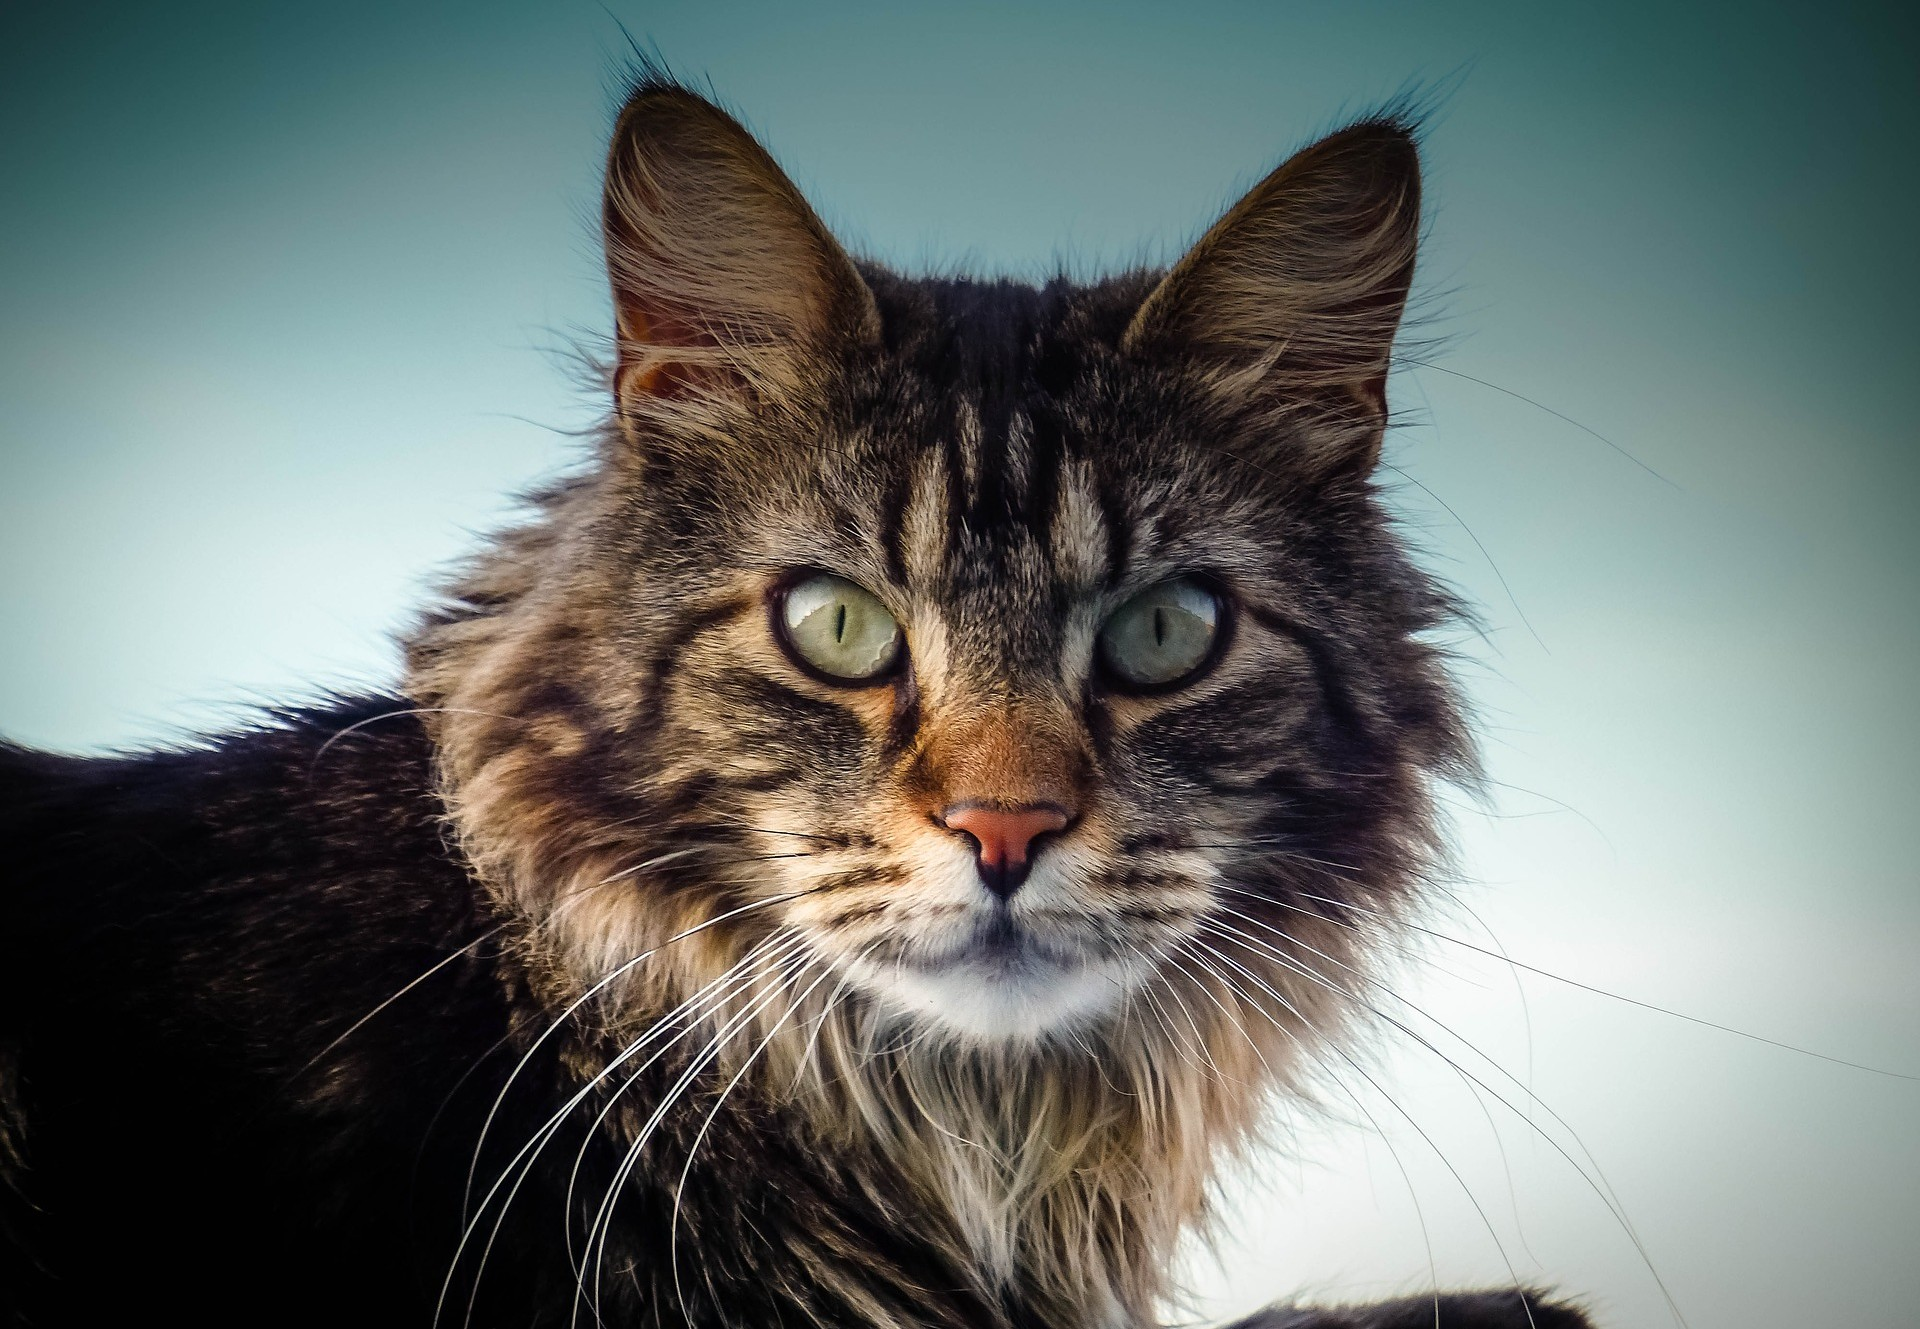
\includegraphics[width=5cm]{cat.jpg} & 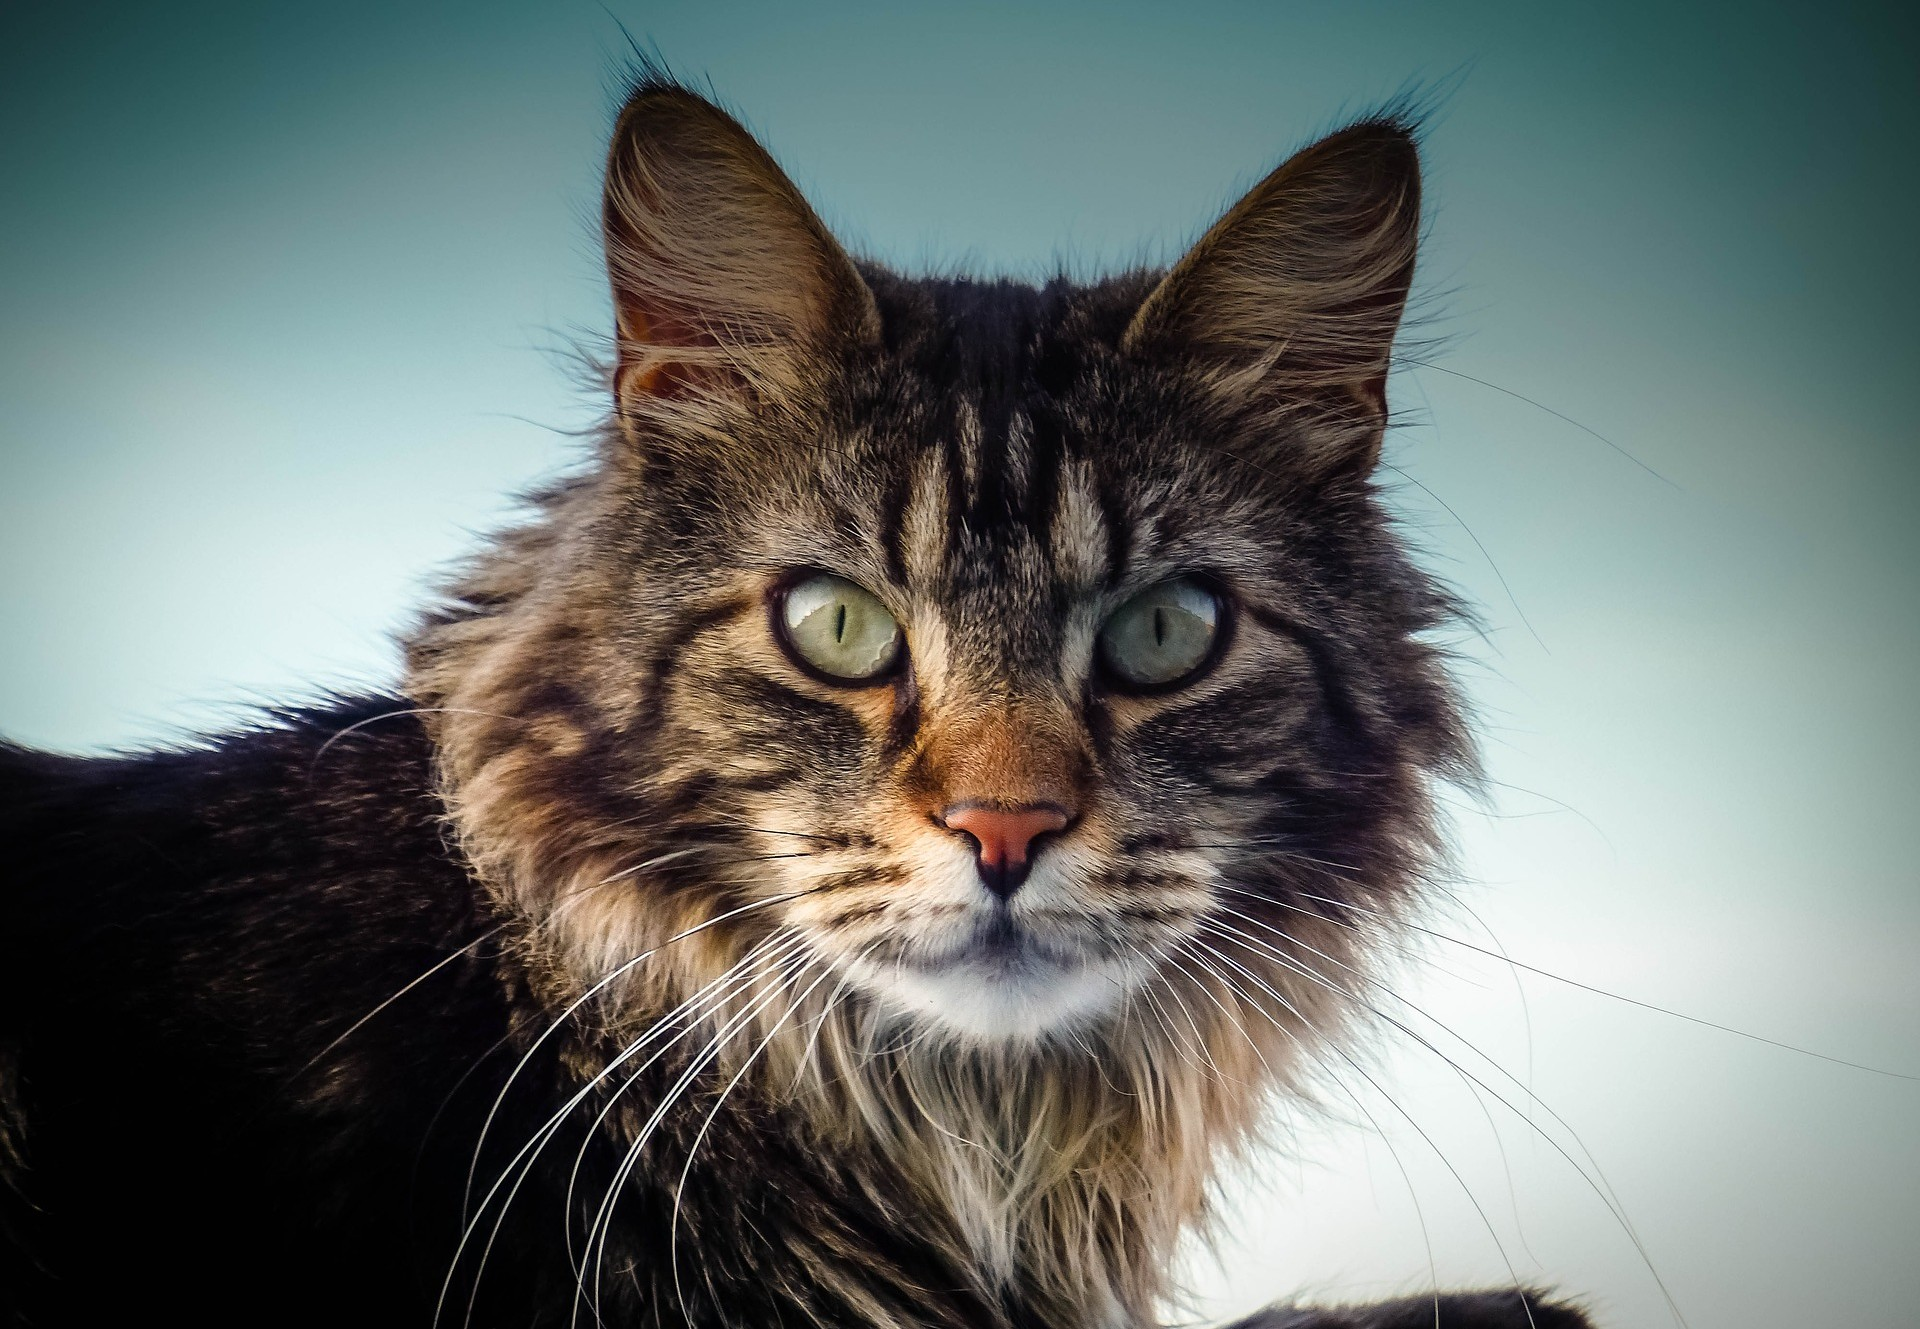
\includegraphics[angle=45,width=5cm]{cat.jpg} \\ \hline
    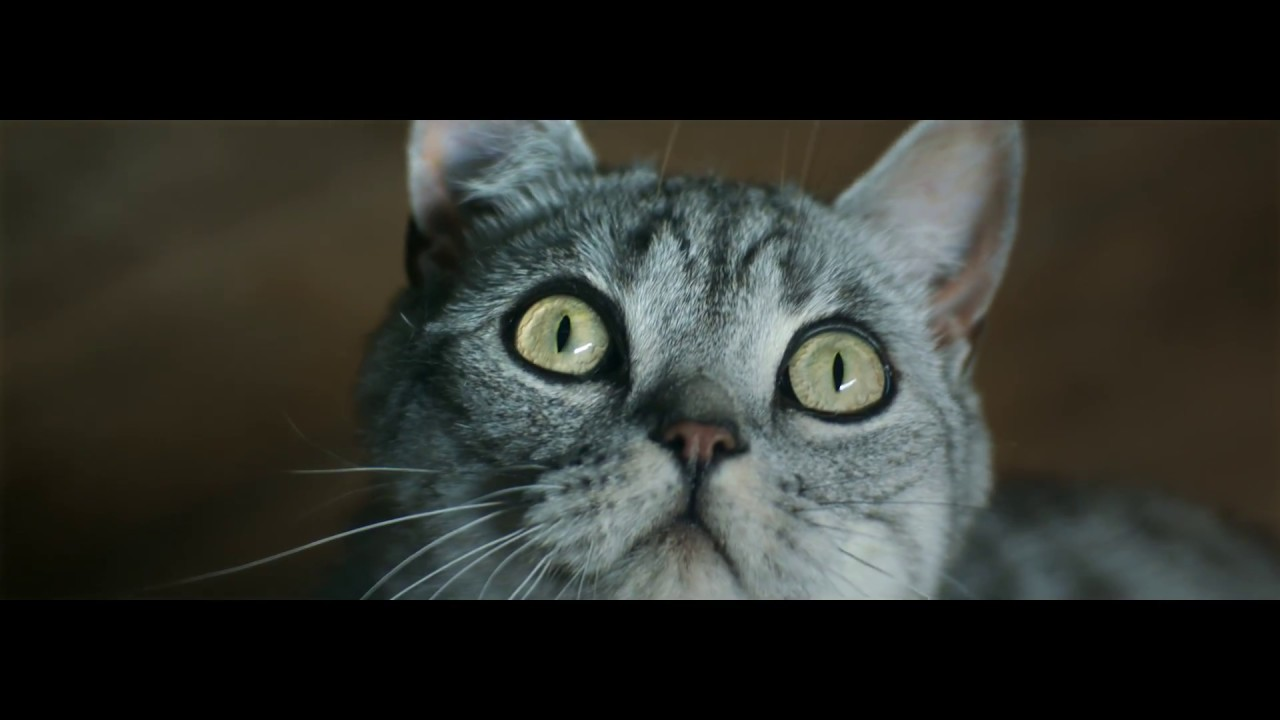
\includegraphics[width=5cm]{cat2.jpg} & 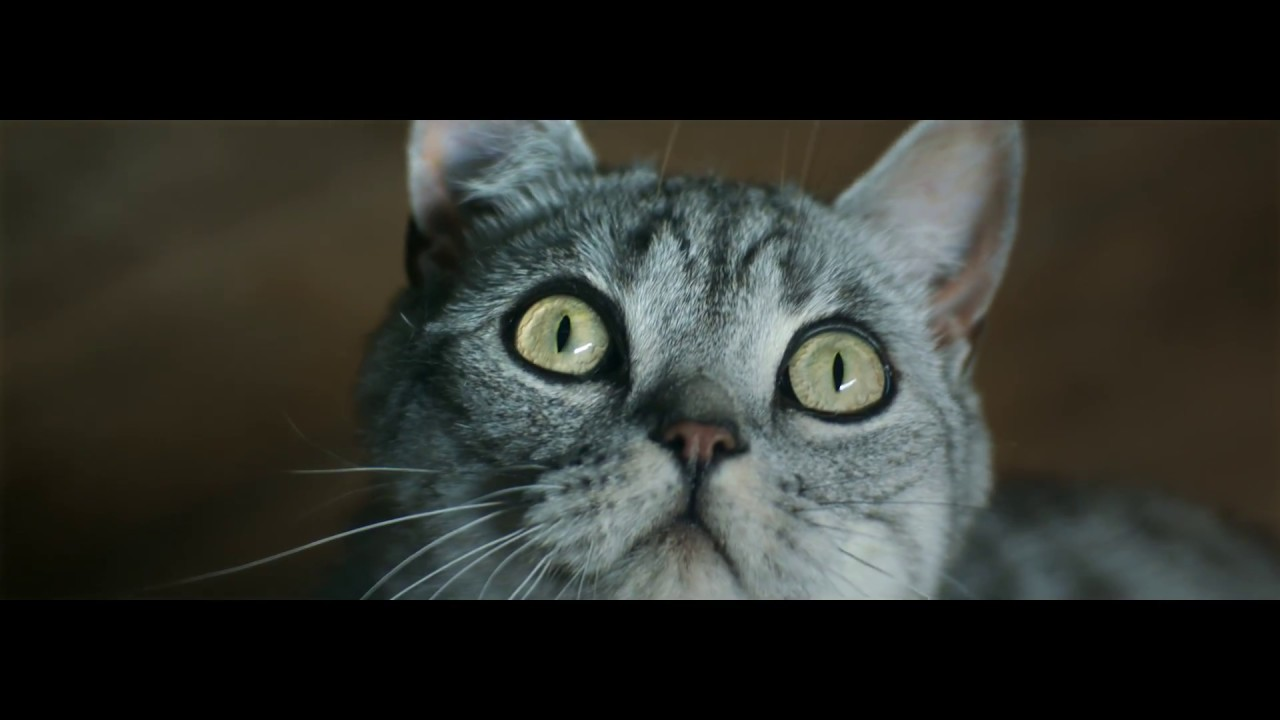
\includegraphics[width=2.5cm]{cat2.jpg} \\ \hline
  \end{tabular}
\end{center}

\end{document}
